\chapter{Realisierung}\label{ch:realisierung_der_anwendung}
TODO

\section{Einbindung der Mustererkennung}
In Abschnitt \ref{mustererkennung_vuforia} haben wir uns bereits mit der internen Funktionsweise des Augmented Reality Frameworks \textquote{Vuforia} beschäftigt. 
Damit wir dessen vollen Umfang in der Unity-Projektumgebung nutzen können, mussten wir das entsprechende Vuforia Software Development Kit einbinden.
Es beinhaltet im wesentlichen alle Grundbausteine für die Entwicklung einer Augmented Reality App und stellt diese in Form von Unity Gameobjects bereit. 
Dadurch sind sie genau wie herkömmliche Gameobjects benutzbar. 
Sie können ganz einfach in ein bestehendes Unity-Projekt integriert werden und es erweitern.
Beispiele für ein paar der Bausteine wären zum einen die AR Camera. 
Sie beinhaltet Logik um die Hauptkamera des ausführenden Gerätes anzusteuern. Die Szene in der die Kamera platziert wurde wird nun durch die Sicht des Gerätes dargestellt. 
Dieser Baustein ist essentiell für die Erstellung einer Augmented Reality App. 

Auf einen Weiteren essentiellen Baustein aus der Vuforia SDK wird in den nachfolgenden Unterabschnitten \ref{image_targets} und \ref{integration_image_targets} eingegangen. 

\subsection{Image Targets}\label{image_targets}
\subsection{Integration der Image Targets}\label{integration_image_targets}

\section{Verwendung von 3D Objekten}
Die in der Anwendung verwendeten 3D Objekte liegen im \textquote{object}-Format vor, welches durch die Dateiendung \textquote{.obj} gekennzeichnet ist. 
Dem Dateiformat liegt das polygonale Modell zugrunde, das 3D Objekte als Zusammensetzung von Polygonen, die wiederum aus durch Kanten verbundenen Koordinaten bestehen, definiert. 
Die geläufigsten so entstehenden Polygonnetze sind Dreiecksnetze und Vierecksnetze.

In einer  \textquote{.obj}-Datei sind somit die Koordinaten von Punkten im dreidimensionalen Raum definiert, welche über Kantendefinitionen zu Flächen verbunden werden. 
Um 3D Objekte realistisch erscheinen zu lassen, findet der Prozess des sogenannten \textquote{Texture Mappings} statt, in welchem eine Textur im Bildformat über ein 3D Objekt gelegt wird. 
Auf Codebasis wird dies realisiert, indem in der \textquote{.obj}-Datei zweidimensionale Texturkoordinaten für eine vorhandene Textur definiert und bestimmten Punktkoordinaten des Objekts zugewiesen werden.

Primitive 3D Objekte, die aus wenigen Polygonen bestehen, können somit leicht selbst erstellt werden, während die Erstellung von komplexeren Objekten und zugehörigen Texturen mehr Zeitaufwand erfordert. 
Da dieser Zeitaufwand nicht in den zeitlichen Rahmen dieses IT Projektes gepasst hat, haben wir uns dafür entschieden, kostenlose 3D Objekte mit zugehörigen Texturen von verschiedenen Anbietern aus dem Internet zu verwenden, welche im folgenden aufgelistet sind.

\begin{itemize}
\item https://www.turbosquid.com/
\item https://www.cgtrader.com/
\item https://free3d.com/
\end{itemize}

Wie bereits in Kapitel \ref{projektziel} erwähnt, sollen die Länder, die in der App enthalten sind durch passende 3D Objekte repräsentiert werden, welche auf das erkannten Image Target eines Landes gerendert werden. 
Die folgende Auflistung zeigt die gewählten 3D Objekte für ihre zugehörigen Länder, gegliedert in Kontinente. Diese sind bildlich auch im Anhang dargestellt.

\textbf{3D Objekte für Afrika:}
\begin{itemize}
\item Kongo: Affe
\item Südafrika: Elefant
\item Ägypten: Pyramide
\end{itemize}

\textbf{3D Objekte für Europa:}
\begin{itemize}
\item Deutschland: Brandenburger Tor	
\item Frankreich: Eiffelturm
\item Niederlande: Windmühle
\end{itemize}

\textbf{3D Objekte für Nordamerika:}
\begin{itemize}
\item Kanada: Hirsch
\item USA: Empire State Building
\item Mexico: Maya Tempel
\end{itemize}

\textbf{3D Objekte für Südamerika:}
\begin{itemize}
\item Brasilien: Palmenwald
\item Argentinien: Pinguine
\item Peru: Machu Picchu
\end{itemize}

\textbf{3D Objekte für Asien:}
\begin{itemize}
\item Indien: Taj Mahal
\item Malaysia: Petrona Towers
\item Japan: Tempel
\end{itemize}

Die Einbindung dieser 3D Objekte und die dazu nötige Vorverarbeitung dieser werden in den folgenden Kapiteln beschrieben.
\subsection{Vorverarbeitung}
Die Vorverarbeitung der 3D Objekte wurde mit dem kostenlosen Grafikprogramm \textquote{Blender} realisiert, welches einen großen Funktionsumfang für die Bearbeitung und Erstellung von 3D Körpern bietet. 

Die vorherige Bearbeitung der 3D Objekte war hauptsächlich aus zwei Gründen nötig. 
Zum Einen erleichterte sie die Einbindung der Objekte, da die aus unterschiedlichen Quellen stammenden 3D Objekte meist sehr groß skaliert und rotiert waren.
Durch einfache Transformationsoperationen konnten diese Objekte somit auf eine einheitliche Größe und Ausrichtung normalisiert werden, wodurch die aufwendigere Bearbeitung in Unity nicht mehr nötig war.

Ein weiterer Anwendungsfall für die nötige Vorverarbeitung der 3D Objekte in Blender war die nötige Reduktion der Polygonzahl der Objekte. 
Die aus dem Internet stammenden Körper wiesen eine sehr hohe Polygonzahl vor und waren dadurch sehr hoch aufgelöst, was zu einer größeren Dateigröße und somit einer Belastung des Anwendungsspeichers führen würde. 
Eine solch hohe Auflösung war in unserem Anwendungsfall nicht nötig, da die 3D Objekte auf dem Globus sehr klein skaliert angezeigt werden und die gegebenen Genauigkeiten somit nicht auffallen würden. 
Um Speicherplatz innerhalb der App zu sparen wurde die Polygonzahl und damit die Dateigröße der 3D Objekte mithilfe von Blender um das zehnfache verringert, bevor diese in der App eingebunden wurden.

Die Veränderung der Polygonzahl wird durch Grafiken \ref{fig:elefant_viele_polygone} und \ref{fig:elefant_wenig_polygone} dargestellt.

\begin{figure}[!htb]
\minipage{0.48\textwidth}
  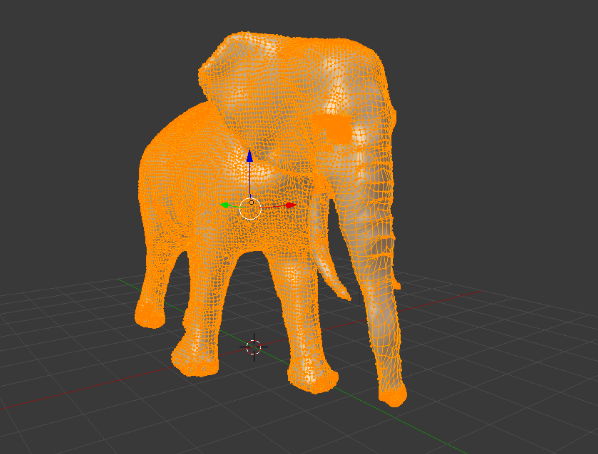
\includegraphics[width=\linewidth]{elefant_viele_polygone.png}
  \caption{Polygonnetz vor Bearbeitung}\label{fig:elefant_viele_polygone}
\endminipage\hfill
\minipage{0.48\textwidth}
  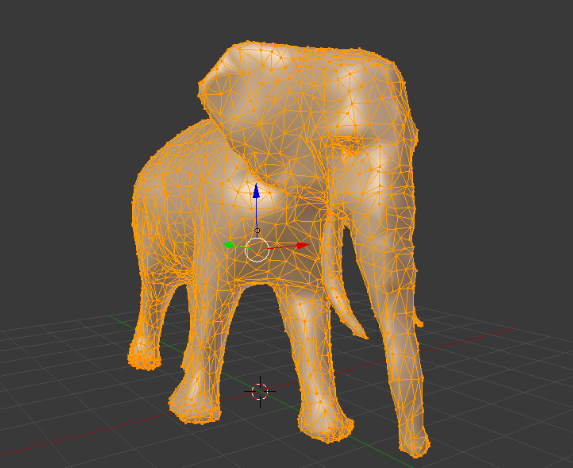
\includegraphics[width=\linewidth]{elefant_wenig_polygone.png}
  \caption{Polygonnetz nach Bearbeitung}\label{fig:elefant_wenig_polygone}
\endminipage\hfill
\end{figure}

Aus Grafik \ref{fig:elefant_wenig_polygone} geht hervor, dass sich die Gestalt des 3D Objektes trotz verringerter Polygonzahl kaum verändert und der Prozess der Polygonreduktion somit zu einem nicht merklichen Genauigkeitsverlust führt.
\subsection{Einbindung der 3D Objekte in Unity}
Der Zugriff auf die ausgewählten 3D Objekte innerhalb des Unity-Entwicklungsoberfläche, sowie der Applikation wird ermöglicht, indem die Objekte im Projektpfad als Ressourcen abgelegt werden, welche beim Bauen der Applikation auf das Endgerät mit übertragen werden. 

Wie in Kapitel, \ref{projektziel} beschrieben, soll ein 3D Objekt nur bei der Erkennung des ihm zugeordneten Landes angezeigt werden.
Um dies zu realisieren, werden die 3D Objekte in der Entwicklungsoberfläche als Kind-Objekte der in Kapitel \ref{integration_image_targets} beschriebenen Image-Targets angelegt.
Das Verhalten dieser Vuforia-Elemente wird durch das \textquote{DefaultTrackableEvent-Handler}-Skript bestimmt, welches den Elementen standardmäßig beigefügt ist. 
Bei der Feuerung des \textquote{OnTrackableFound}-Events, das heißt der Erkennung eines Image-Targets, werden die diesem untergeordneten, renderbaren Kindelemente mithilfe der von Unity bereitgestellten \textquote{Renderer}-Klasse automatisch gerendert.

Das beschriebene \textquote{DefaultTrackable-EventHandler}-Skript kann nach belieben bearbeitet werden, um ein besonderes, durch den Benutzer gewünschtes Verhalten hervorzurufen.
In unserem Fall wurde das \textquote{OnTrackable-Found}-Event so überschrieben, dass zusätzlich zu dem 3D Objekt noch zwei Buttons angezeigt werden, mit welchen der User interagieren kann.

\section{Verwaltung der Daten}
\subsection{Datenbankentwurf}\label{datenbankentwurf}
\subsection{Zugriff auf Datenbankinhalte}

\section{Realisierung der Anwendung in Unity}
\subsection{Informationsbereich}
\subsection{Quizbereich}
